\question{\bfseries Finding Peep Chan}

\subsection*{\sectionfont\upshape Background}

เด็กหญิงเกดเป็นเด็กน้อยแสนน่ารักที่เลี้ยงแมวเหมียวชื่อว่าปิ๊บจัง วันหนึ่งเจ้าปิ๊บจังหายไปเลยออกไปตามหา 
เด็กหญิงเกดได้เบาะแสมาว่าเจ้าปิ๊บจังไปติดอยู่ในถ้ำแห่งหนึ่ง ถ้ำมีลักษณะเป็น grid 2 มิติ 
แบ่งเป็นห้องขนาด $N \times M$ โดยห้องซ้ายบนสุดคือพิกัด $(1,1)$ และห้องขวาล่างสุดคือพิกัด $(N,M)$

แต่ละห้องจะสามารถเดินไปมาหาสู่กันได้เฉพาะห้องที่ติดกันในทิศทาง บน ล่าง ซ้าย ขวา หรือก็คือ 
ห้อง $(x,y)$ สามารถเดินไปยังห้อง $(x-1,y)$, $(x+1,y)$, $(x,y-1)$ และ $(x,y+1)$ 
นอกจากนี้ในถ้ำยังมีทางลัดอีก $K$ เส้นทาง โดยเส้นทางที่ $i$ 
จะสามารถเดินทางไปมาหาสู่กันระหว่างห้อง $(x_{i1},y_{i1})$ และ $(x_{i2},y_{i2})$ ได้\;
การเดินทางไปยังช่องที่ติดกันในทิศทาง บน ล่าง ซ้าย ขวา หรือ การใช้ทางลัด 
แต่ละครั้งจะใช้เวลาในการเดินทาง 1 วัน (ขอเรียกระยะการเดินของแมวใน 1 วันว่า 1 แมวเดิน)

\begin{center}
    \bigskip
    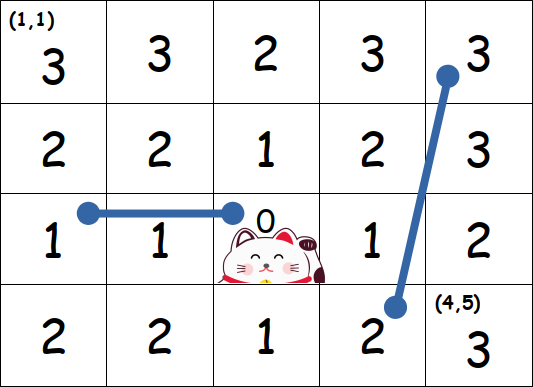
\includegraphics[width=0.7\linewidth]{figures/coding_national_findingpeepchan_01.png}
\end{center}

จากรูปแสดงระยะทางในหน่วยแมวเดิน จากการเดินของแมวที่อยู่ที่ห้องตรงกลาง ลูกศรคือเส้นทางลัด

เด็กหญิงเกดรู้สึกจนปัญญามากเพราะไม่รู้ว่าแมวอยู่ห้องไหนในถ้ำกันแน่ ดังนั้นจะถือว่า \\
\uline{ตอนแรกแมวมีโอกาสที่จะอยู่ในแต่ละห้องด้วยความน่าจะเป็นที่เท่า ๆ กัน} 
(ซึ่งมีค่าเท่ากับ $\frac{1}{N \times M}$) เด็กหญิงเกดจึงไปร้องขอต่อเทพเจ้าให้ช่วยเหลือ

\medskip
เทพเจ้ามีพลังวิเศษ 2 อย่าง คือ
\begin{itemize}
\item \textbf{หยั่งรู้} --- เทพเจ้าจะเลือกห้องห้องหนึ่ง หลังจากนั้นพระเจ้าจะรู้ว่าแมวอยู่ห่างจากห้องที่เลือกเป็น
    ``ระยะทางที่ใกล้ที่สุด'' กี่แมวเดิน แต่ว่าสามารถใช้ได้วันละ 1 ครั้งเท่านั้น
\item \textbf{ช่วยเหลือ} --- เทพเจ้าจะเลือกห้องห้องหนึ่งเพื่อช่วยเหลือแมว 
    ถ้าแมวอยู่ในห้องที่เลือกจะถือว่าช่วยเหลือสำเร็จ แต่ว่าสามารถใช้ได้แค่ครั้งเดียวเท่านั้น
\end{itemize}

เนื่องจากถ้ำมีอากาศอยู่เบาบางมาก แมวจะสามารถมีชีวิตอยู่ได้แค่ 2 วัน 
เพราะฉะนั้นการช่วยเหลือแมวจะมีโอกาสแค่วันนี้กับพรุ่งนี้เท่านั้น

\newpage
เทพเจ้าตอบรับคำร้องขอของเด็กหญิงเกด และดำเนินการช่วยเหลือตามขั้นตอนต่อไปนี้
\begin{enumerate}
\item เทพเจ้าจะใช้พลัง \textbf{“หยั่งรู้”} เพื่อเลือกห้องห้องหนึ่งในถ้ำ
\item เทพเจ้าจะพิจารณาว่า จะใช้พลัง \textbf{“ช่วยเหลือ”} ในวันนี้เลยหรือไม่ 
    แน่นอนว่าถ้าใช้แล้วจะไม่สามารถดำเนินการในข้อต่อไปได้ 
    เพราะไม่สามารถใช้พลัง \textbf{“ช่วยเหลือ”} ได้อีกต่อไป
\item ในกรณีที่เทพเจ้าไม่ได้ใช้พลัง \textbf{“ช่วยเหลือ”} เทพเจ้าจะนอน 1 วันเพื่อพักผ่อน 
    ในขณะที่เทพเจ้านอนพัก แมวจะเคลื่อนที่ 1 ครั้ง 
    โดยการเคลื่อนที่นี้แมวจะสามารถเดินไปยังห้องที่ติดกันหรือห้องที่มีทางลัดไปหากันได้ 
    โดย\uline{แมวจะเดินไปยังห้องที่ไปได้ทั้งหมดด้วย} \uline{โอกาสที่เท่าๆกัน}
\item ในวันถัดไป เทพเจ้าก็จะใช้พลัง \textbf{“หยั่งรู้”} อีกครั้ง
\item เทพเจ้าก็จะใช้พลัง \textbf{“ช่วยเหลือ”} เพราะว่าเป็นโอกาสสุดท้ายที่จะช่วยเหลือแมวแล้ว
\end{enumerate}

\subsection*{\sectionfont\upshape Problem Statement}

เทพเจ้าอยากทราบว่า ความน่าจะเป็นที่มากที่สุดที่เป็นไปได้ที่จะช่วยเหลือแมวได้สำเร็จเป็นเท่าไหร่ 
ถ้าดำเนินการช่วยเหลืออย่าง optimal ที่สุด

\subsection*{\sectionfont\upshape Program Specification}

โปรแกรมที่คุณเขียนจะต้องอ่านข้อมูลจาก stardard input 
และเขียนคำตอบลง standard output โดยข้อมูลจะมีฟอร์แมตดังต่อไปนี้

\bigskip\noindent
{\sectionfont\bfseries Input Format}
\begin{itemize}
\item บรรทัดแรกประกอบด้วยจำนวนเต็ม $N, M$ แทนขนาดของถ้ำ และ K แทนจำนวนเส้นทางลัด
\item K บรรทัดถัดมา บรรทัดที่ $i$ จะประกอบด้วย จำนวนเต็ม 4 จำนวน 
    $x_{i1}$, $y_{i1}$, $x_{i2}$ และ $y_{i2}$ คั่นด้วยช่องว่าง ซึ่งระบุเส้นทางลัดเส้นที่ $i$
\begin{lstlisting}
N M K
x_{1,1} y_{1,1} x_{1,2} y_{1,2}
x_{2,1} y_{2,1} x_{2,2} y_{2,2} <%\SuppressNumber\AlternateNumber{...}%>
                                <%\AlternateNumber{K+1}%>
x_{K,1} y_{K,1} x_{K,2} y_{K,2} <%\ReactivateNumber%>
\end{lstlisting}
\textbf{หมายเหตุ:} รับประกันว่า $1 \leq x_{i1}, x_{i2} \leq N$ และ 
$1 \leq y_{i1},y_{i2} \leq M$ และจะไม่มีเส้นทางลัดซ้ำกัน และไม่มีทางลัดของห้องที่อยู่ติดกัน
\end{itemize}

\medskip\noindent
{\sectionfont\bfseries Output Format}
\begin{itemize}
    \item ตอบเป็นจำนวนจริง 1 จำนวน แทนความน่าจะเป็นที่มากที่สุดที่เป็นไปได้ของการช่วยเหลือแมว
    ถ้าเทพเจ้าทำการช่วยเหลืออย่าง Optimal ที่สุด \\
    (\textbf{หมายเหตุ:} คำตอบจะถูกต้องถ้าคาดเคลื่อนไม่มากกว่าคำตอบจริงเกิน $10^{-6}$)
\end{itemize}

\newpage
\subsection*{\sectionfont\upshape First Data Example}
\begin{tabular}{p{0.45\linewidth}p{0.45\linewidth}}
\toprule
Example Input & Example Output \\
\midrule
\ttfamily\setstretch{0.8}
2 2 1 \newline
1 1 2 2 &
\ttfamily\setstretch{0.8}
0.9166666667 \\
\bottomrule
\end{tabular}

\medskip\noindent
\textbf{อธิบายตัวอย่างที่ 1:} จากตัวอย่างของข้อมูลนำเข้าข้างต้น สามารถแสดงให้เห็นตามรูปที่ปรากฏทางด้านข้าง
โดยที่ลูกศรแสดงเส้นทางลัดระหว่างห้องสองห้อง
\marginnote{%
    \centering
    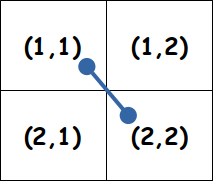
\includegraphics[width=0.7\linewidth]{figures/coding_national_findingpeepchan_02.png}
}

หนึ่งในการวิธีช่วยเหลือที่ optimal ขอเทพเจ้ามีดังต่อไปนี้
\begin{enumerate}
\item วันแรก ใช้พลัง \textbf{“หยั่งรู้”} ที่ห้อง $(1,2)$
    \begin{enumerate}
        \item ความน่าจะเป็น $\frac{1}{4}$ ที่ระยะทางที่ใกล้ที่สุด 
            จะเป็น $0$ แมวจะอยู่ที่ห้อง $(1,2)$ \\
            กรณีนี้สามารถใช้พลัง \textbf{“ช่วยเหลือ”} เพื่อช่วยแมวได้ทันที
        \item ความน่าจะเป็น $\frac{2}{4}$ ที่ระยะทางที่ใกล้ที่สุด 
            จะเป็น 1 แมวอาจจะอยู่ที่ห้อง $(1,1)$ \\
            หรือ $(2,2)$ ก็ได้\; กรณีนี้ควรรอวันที่ 2
        \item ความน่าจะเป็น $\frac{1}{4}$ ที่ระยะทางที่ใกล้ที่สุด 
            จะเป็น 2 แมวจะอยู่ที่ห้อง $(2,1)$ \\
            กรณีนี้สามารถใช้พลัง \textbf{“ช่วยเหลือ”} เพื่อช่วยแมวได้ทันที
    \end{enumerate}
\item จากข้อ 1{\hrsp}(b) ระหว่างวันในขณะที่เทพเจ้านอนพัก การเคลื่อนที่ของแมวเป็นดังนี้
    \begin{itemize}
        \item ความน่าจะเป็นที่แมวจะเดินไปห้อง $(1,2)$ คือ 
            $\frac{2}{4}\times\frac{1}{3}=\frac{2}{12}$ \\ 
            ← เดินจาก $(1,1)$ หรือ $(2,2)$
        \item ความน่าจะเป็นที่แมวจะเดินไปห้อง $(1,1)$ คือ 
            $\frac{1}{4}\times\frac{1}{3}=\frac{1}{12}$ ← เดินจาก $(2,2)$
        \item ความน่าจะเป็นที่แมวจะเดินไปห้อง $(2,2)$ คือ 
            $\frac{1}{4}\times\frac{1}{3}=\frac{1}{12}$ ← เดินจาก $(1,1)$
        \item ความน่าจะเป็นที่แมวจะเดินไปห้อง $(2,1)$ คือ 
            $\frac{2}{4}\times\frac{1}{3}=\frac{1}{12}$ \\
            ← เดินจาก $(1,1)$ หรือ $(2,2)$
    \end{itemize}
\item วันถัดมาวันที่ ใช้พลัง “หยั่งรู้” ที่ห้อง $(1,2)$ เช่นเดิม
    \begin{enumerate}
        \item ความน่าจะเป็น $\frac{2}{12}$ ที่ระยะทางที่ใกล้ที่สุดจะเป็น 0 
            แมวจะอยู่ที่ห้อง $(1,2)$ \\
            กรณีนี้สามารถชใช้พลัง \textbf{“ช่วยเหลือ”} แมวได้แน่นอน
        \item ความน่าจะเป็น $\frac{2}{12}$ ที่ระยะทางที่ใกล้ที่สุดจะเป็น 2 
            แมวจะอยู่ที่ห้อง $(2,1)$ \\
            กรณีนี้สามารถใช้พลัง \textbf{“ช่วยเหลือ”} แมวได้แน่นอน
        \item ความน่าจะเป็น $\frac{1}{12}+\frac{1}{12}=\frac{2}{12}$ 
            ที่ระยะทางที่ใกล้ที่สุดจะเป็น 1 
            แมวจะอาจจะอยู่ที่ห้อง $(1,1)$ หรือ $(2,2)$ ก็ได้ \\
            กรณีนี้ การเลือกห้องใดห้องหนึ่งเพื่อใช้พลัง \textbf{“ช่วยเหลือ”} 
            จะมีโอกาสช่วยแมวสำเร็จด้วยความน่าจะเป็น $\frac{2}{12} \times \frac{1}{2}=\frac{1}{12}$
    \end{enumerate}
\item สรุปว่า ความน่าจะเป็นที่เทพเจ้าจะสามารถช่วยเหลือแมวได้ ตามข้อ 1{\hrsp}(a), 1{\hrsp}(c), 
    3{\hrsp}(a), 3{\hrsp}(b) และ 3{\hrsp}(c) คือ
    \[
        \frac{1}{4} + \frac{1}{4} + \frac{2}{12} + \frac{2}{12} + \frac{1}{12} 
        = \frac{11}{12} \approx 0.9166666667
    \]
\end{enumerate}


\subsection*{\sectionfont\upshape Second Data Example}
\begin{tabular}{p{0.45\linewidth}p{0.45\linewidth}}
\toprule
Example Input & Example Output \\    
\midrule
\ttfamily\setstretch{0.8}
3 3 3 \newline
3 1 1 2 \newline
3 1 2 3 \newline
1 2 3 1 &
\ttfamily\setstretch{0.8} 
0.7259259259 \\
\bottomrule
\end{tabular}

\subsection*{\sectionfont\upshape Constraints}

โปรแกรมของคุณจะถูกทดสอบกับ test cases สองชุด (เรียกว่าชุดเล็ก และชุดใหญ่)
\begin{itemize}
\item test cases ชุดเล็กจะมีเงื่อนไข ขนาดของถ้ำสอดคล้องกับเงื่อนไข 
    $1 \leq N,M \leq 20$ และ $N \times M \leq 200$ 
    และจำนวนเส้นทางลัดสอดคล้องกับเงื่อนไข $1 \leq K \leq 100$
\item test cases ชุดใหญ่จะมีเงื่อนไขว่า ขนาดของถ้ำสอดคล้องกับเงื่อนไข 
    $1 \leq N,M \leq 20$ และจำนวนเส้นทางลัดสอดคล้องกับเงื่อนไข $1 \leq K \leq 70,000$
\end{itemize}
